\documentclass[a4paper, 11pt, titlepage]{book}
\usepackage{fancyhdr}
\usepackage{graphicx}
\usepackage{imakeidx}
\usepackage{makeidx}
\usepackage{mathtools}
\usepackage[spanish]{babel}
\usepackage{eurosym}
\usepackage{hyperref}
\usepackage{amssymb}
\usepackage{listings}
\usepackage{xcolor}

\setcounter{secnumdepth}{5}
\setcounter{tocdepth}{5}

\title{Diario}
\author{Francisco Javier Balón Aguilar}

\begin{document}

\maketitle
\renewcommand{\contentsname}{Índice}
\tableofcontents
\newpage

\chapter{El Administrador}

    \section{Watchdog}

    El watchdog (perro guardían o vigilante) del kernel de Linux se utiliza para 
    monitorizar y vigilar un sistema que se está ejecutando, de forma que pueda 
    ser reiniciado automáticamente en caso de fallo de software irrecuperables.

    El módulo de watchdog es específico para el hardware o chip que se utiliza.

    Los usuarios, por norma general, no necesitan de vigilancia en sus sistemas, 
    pues pueden ellos mismos restablecer el sistema manualmente; así está pensado
    para dispositivos críticos que requieran de restablecimientos sin intervención
    humana, por ejemplo servidores en una ubicación remota o equipos integrados 
    en naves espaciales.

    En su intervención es necesario proceder con precaución, ya que configuraciones
    incorrectas o erróneas podrían provocar:

    \begin{itemize}
        \item Bucles infinitos de reinicios.
        \item Corrupción de archivos debido al hard reset.
        \item Reinicios aleatorios impredecibles.
    \end{itemize}

    Por lo que es preferible evitar el uso de servidores en vivo para probar el 
    funcionamiento de watchdog.

    \subsection{Watchdog module}

        La funcionalidad de watchdog sobre hardware configura un temporizador 
        que agota el tiempo de espera después de un período predeterminado.
        El software de watchdog actualiza periódicamente el temporizador del 
        hardware, y si éste deja de actualizarse luego del período establecido 
        el temporizador realizará un restablecimiento de hardware del dispositivo.
        Para que un temporizador watchdog sea funcional, el fabricante de la placa 
        base tiene que permitir esta funcionalidad en el chip.

        A menudo, la documentación del fabricante de hardware no deja claro 
        sobre si se implementó o no esta funcionalidad. En ese caso hay que 
        testearlo directamente.

        Además es necesario el módulo del kernel de vigilancia correcto, que será 
        cargado en el sistema Linux. Diferentes chips utilizan diferentes módulos,
        por ejemplo:

        \begin{itemize}
            \item Intel utiliza \textit{iTCO\_wdt}.
            \item El hardware de HP utiliza \textit{hpwdt}.
            \item Los mainframes de IBM utilizan \textit{vmwatchdog}.
            \item Xen VM utiuliza \textit{xen\_wdt}.
        \end{itemize}

        Una vez corroborado la carga del módulo es posible verificar \textit{/dev/watchdog}
        en el sistema Linux. Si el archivo está presente, significa que se cargó el controlador.
        El sistema escribe periódicamente a \textit{/dev/watchdog} (esta acción
        suele llamarse coloquialmente <<patear o alimentar al perro guardián>> / <<kicking
        or feeding the watchdog>>). Si el sistema falla y no patea o alimenta al 
        perro, el sistema se restablecerá completamente.

    \subsection{Watchdog daemon}

        El demonio de watchdog abre el dispositivo y proporciona la actualización 
        necesaria para evitar que el sistema se restablezca. Éste puede comprobar 
        el espacio de la tabla de procesos, el uso de memoria (memory usage), la 
        accesibilidad de archivos, la carga de trabajo, desbordamientos en la tabla de 
        archivos, ping a direcciones IP, tráfico de interfaz de red, temperatura, 
        procesos en ejecución, etc. Como ya hemos visto, si las pruebas fallan 
        el perro provocará el apagado.

    \subsection{Iniciando y parando el demonio de watchdog}

        El demonio de watchdog debería iniciarse en el momento del arranque. 
        Podemos verificar si está iniciado con:

        \begin{lstlisting}[language=bash]
    ps -af | grep watch*\end{lstlisting}

        Si el kernel no estuviera compilado con \textit{CONFIG\_WATCHDOG\_NOWAYOUT}
        y cerramos correctamente \textit{/dev/watchdog} no habrá reinicio. Podemos 
        escribir un carácter $V$ en \textit{/dev/watchdog} y luego cerrar el archivo;
        lo que detendrá al perro guardián.

        \subsubsection{Testeando watchdog} Si queremos comprobar que el control de 
        hardware está funcionando, podemos lanzar la siguiente orden con privilegios 
        root:

        \begin{lstlisting}[language=bash]
    cat >> /dev/watchdog\end{lstlisting}

        Una vez haya pasado el tiempo esperado, dependiendo de la configuración 
        del kernel, el sistema realizará el hard reboot.

    \subsection{Configuración del demonio de watchdog}

        Una vez conocemos watchdog, podemos iniciar su configuración. El fichero de 
        configuración de watchdog se encuentra en \textit{/etc/watchdog.conf} 
        (es posible que haya que instalar el paquete \textit{watchdog} en la distribución 
        utilizada).

        \begin{lstlisting}[language=bash]
    # cat /etc/watchdog.conf
    realtime = yes
    priority = 1\end{lstlisting}

\chapter{El Ingeniero}

\chapter{El Programador}

    \section{El programador C}

    \section{El programador C\#}

    \section{El programador Java}

    \section{El programador Python}

\chapter{El Hacker}

    \section{Reconocimiento}
            
        \subsection{nmap}

            % https://nmap.org/man/es/man-host-discovery.html

            \subsubsection{-sL (Sondeo de lista)} El sondeo de lista es un tipo de descubrimiento
            de sistemas que tan solo lista cada equipo de la/s red/es especificada/s, sin enviar paquetes 
            de ningún tipo a los objetivos. Por omisión, Nmap va a realizar una resolución inversa DNS en 
            los equipos, para obtener sus nombres. Es sorprendente cuanta información útil se puede obtener 
            del nombre de un sistema. Por ejemplo fw.chi.playboy.com es el cortafuegos de la oficina en 
            Chicago de Playboy Enterprises. Adicionalmente, al final, Nmap reporta el número total de 
            direcciones IP. El sondeo de lista es una buena forma de asegurarse de que tenemos las 
            direcciones IP correctas de nuestros objetivos. Si se encontraran nombres de dominio que no 
            reconoces, vale la pena investigar un poco más, para evitar realizar un análisis de la red 
            de la empresa equivocada.

            Ya que la idea es simplemente emitir un listado de los sistemas objetivo, las opciones de 
            mayor nivel de funcionalidad como análisis de puertos, detección de sistema operativo, o 
            análisis ping no pueden combinarse con este sondeo. Si desea deshabilitar el análisis ping 
            aún realizando dicha funcionalidad de mayor nivel, compruebe la documentación de la opción -P0.

            \subsubsection{-sP (Sondeo ping)} Esta opción le indica a Nmap que únicamente realice 
            descubrimiento de sistemas mediante un sondeo ping, y que luego emita un listado de los equipos 
            que respondieron al mismo. No se realizan más sondeos (como un análisis de puertos o detección 
            de sistema operativo). A diferencia del sondeo de lista, el análisis ping es intrusivo, ya que 
            envía paquetes a los objetivos, pero es usualmente utilizado con el mismo propósito. Permite 
            un reconocimiento liviano de la red objetivo sin llamar mucho la atención. El saber cuántos 
            equipos se encuentran activos es de mayor valor para los atacantes que el listado de cada una 
            de las IP y nombres proporcionado por el sondeo de lista.

            De la misma forma, los administradores de sistemas suelen encontrar valiosa esta opción. 
            Puede ser fácilmente utilizada para contabilizar las máquinas disponibles en una red, o 
            monitorizar servidores. A esto se lo suele llamar barrido ping, y es más fiable que hacer 
            ping a la dirección de broadcast, ya que algunos equipos no responden a ese tipo de consultas.

            La opción -sP envía una solicitud de eco ICMP y un paquete TCP al puerto 80 por omisión. 
            Cuando un usuario sin privilegios ejecuta Nmap se envía un paquete SYN (utilizando la llamada 
            connect()) al puerto 80 del objetivo. Cuando un usuario privilegiado intenta analizar objetivos 
            en la red Ethernet local se utilizan solicitudes ARP (-PR) a no ser que se especifique la 
            opción --send-ip.

            La opción -sP puede combinarse con cualquiera de las opciones de sondas de descubrimiento 
            (las opciones -P*, excepto -P0) para disponer de mayor flexibilidad. Si se utilizan cualquiera 
            de las opciones de sondas de descubrimiento y número de puerto, se ignoran las sondas por omisión 
            (ACK y solicitud de eco ICMP). Se recomienda utilizar estas técnicas si hay un cortafuegos con un 
            filtrado estricto entre el sistema que ejecuta Nmap y la red objetivo. Si no se hace así pueden 
            llegar a pasarse por alto ciertos equipos, ya que el cortafuegos anularía las sondas o las 
            respuestas a las mismas.

            \subsubsection{-P0 (No ping)} Con esta opción, Nmap no realiza la etapa de descubrimiento. 
            Bajo circunstancias normales, Nmap utiliza dicha etapa para determinar qué máquinas se encuentran 
            activas para hacer un análisis más agresivo. Por omisión, Nmap sólo realiza ese tipo de sondeos, 
            como análisis de puertos, detección de versión o de sistema operativo contra los equipos que se 
            están «vivos». Si se deshabilita el descubrimiento de sistemas con la opción -P0 entonces Nmap 
            utilizará las funciones de análisis solicitadas contra todas las direcciones IP especificadas. 
            Por lo tanto, si se especifica una red del tamaño de una clase B cuyo espacio de direccionamiento 
            es de 16 bits, en la línea de órdenes, se analizará cada una de las 65.536 direcciones IP. El 
            segundo carácter en la opción -P0 es un cero, y no la letra O. Al igual que con el sondeo de lista, 
            se evita el descubrimiento apropiado de sistemas, pero, en vez de detenerse y emitir un listado de 
            objetivos, Nmap continúa y realiza las funciones solicitadas como si cada IP objetivo se encontrara 
            activa.

    \section{Criptografía}

        \subsection{GnuPG (gpg)}
    
            GnuPG, a veces denominado simplemente gpg (siglas de GNU Privacy Guard) es un derivado libre
            de PGP. Su utilidad es la de cifrar y firmar digitalmente. gpg soporta tanto cifrado simétrico 
            como cifrado asimétrico.
    
            gpg tiene un repositorio de claves, llamado \textbf{anillo de claves} 
            donde almacena todas las claves que tenemos en nuestro sistema; sean privadas o públicas.
    
            Los \textbf{servidores de claves} ayudan a difundir las claves públicas 
            de forma que podamos compartirlas fácilmente para que otros usuarios puedan utilizarlas y
            cifrar con ellas.
    
            \subsubsection{Cifrado simétrico}
    
                El cifrado simétrico es sencillo; se utiliza la misma clave para cifrar y para descifrar.
                Es rápido de procesar y sencillo de usar, como contraposición, tiene la desventaja de la 
                comunicación de la clave\footnote{
                    Tanto $A$ como $B$ deben conocer la misma clave. Por lo que si $A$ cifra un texto con
                    la clave $123$, debe en algún momento comunicarla a $B$ para que éste pueda descifrarla.
                    En esta comunicación encontramos un posible vector de ataque para obtener la clave.
                }.
    
                El uso de gpg con cifrado simétrico es muy sencillo. Simplemente llamamos a un texto sin cifrar
                con el parámetro $-c$ (crypt, cifrar) lo que generará un archivo en formato \textit{.gpg} cifrado
                por defecto con el algoritmo AES con la clave proporcionada (véase figuras \ref{crypt01} y 
                \ref{crypt02}).
    
                \begin{figure}[htp]
                    \centering
                    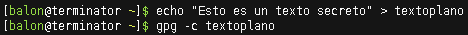
\includegraphics[width=0.8\textwidth]{resources/crypt01.png}
                    \caption{Cifrado simétrico de archivo de texto.}
                    \label{crypt01}
                \end{figure}
    
                \begin{figure}[htp]
                    \centering
                    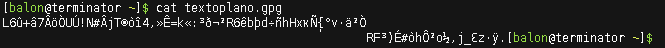
\includegraphics[width=0.8\textwidth]{resources/crypt02.png}
                    \caption{Texto cifrado gpg.}
                    \label{crypt02}
                \end{figure}
    
                Para descifrarlo, simplemente hay que pasarle a gpg el parámetro $-d$ (decrypt, descifrar) y el archivo 
                previamente cifrado (véase figura \ref{decrypt01}).
    
                \begin{figure}[htp]
                    \centering
                    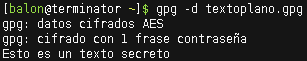
\includegraphics[width=0.5\textwidth]{resources/decrypt01.png}
                    \caption{Texto descifrado con gpg con algoritmo simétrico AES.}
                    \label{decrypt01}
                \end{figure}
    
            \subsubsection{Cifrado asimétrico}
                
                % TODO: genbeta.com/desarrollo/manual-de-gpg-cifra-y-envia-datos-de-forma-segura
    
                \subsubsection{Generación de par de claves}
    
                \subsubsection{Exportación e importación de claves}
    
                \subsubsection{Cifrado con clave pública}
    
                \subsubsection{Descifrado con clave privada}
    
            \subsubsection{Firma digital de archivos}
    
                \paragraph{Verificación y descifrado de archivos firmados}
    
            \subsubsection{Confiabilidad de claves}
    
        \subsection{SSH}
    
            % TODO: solvetic.com/tutoriales/article/1815-el-manual-del-secure-shell/
            \subsubsection{El cliente SSH}
            \subsubsection{El servidor SSH}
            \subsubsection{Securización de SSH}
            \subsubsection{Autenticación mediante intercambio de claves asimétricas (RSA)}
    
                Como ya hemos visto, una conexión común usando el protocolo SSH es de por sí 
                segura; al menos más segura que una conexión no cifrada como telnet, pero presenta,
                \textit{grosso modo} dos inconvenientes:
    
                \begin{enumerate}
                    \item La contraseña, aún yendo cifrada, viaja por la red siempre que nos autenticamos.
                    Esto puede ser peligroso en el caso que haya alguien capturando el tráfico de nuestra 
                    red (\textit{sniffing}) y fuese capaz de descifrar nuestra clave (mediante ataques por 
                    fuerza bruta o diccionario, utilizando alguna vulnerabilidad conocida, etc. Es muy 
                    complicado, pero no imposible).
                    \item En el caso de manejar numerosos servidores y conexiones SSH puede ser muy tedioso 
                    tener que estar recordando contraseñas, almacenandolas, etc. Este método agregaría un plus 
                    de comodidad y escalabilidad a las conexiones.
                \end{enumerate}
    
                La implementación del algoritmo RSA presenta solución a estos problemas. Su funcionamiento
                es:
    
                \begin{enumerate}
                    \item El cliente envía información sobre su clave pública al servidor.
                    \item El servidor busca en su base de datos la clave pública del cliente y, cuando la encuentra,
                    envía al cliente un \textit{challenge} (desafío), que contiene un número aleatorio generado y 
                    cifrado por éste utilizando la clave pública del cliente.
                    \item El cliente recibe el paquete cifrado y usa su clave privada para descifrarlo y devolvérselo 
                    al servidor.
                    \item El servidor comprueba que el número devuelto es el que mandó cifrado, en caso afirmativo, el 
                    usuario se ha autenticado y se le permite la sesión de shell.
                \end{enumerate}
    
                Como observamos, en ningún momento se envían claves por Internet (más que el envío 
                de la clave pública al servidor en el primer contacto, para que éste la conozca). Por 
                supuesto si alguien accede a nuestro equipo y nos roba la clave privada podría autenticarse 
                como nosotros y suplantar nuestra identidad criptográfica. Por esta razón es necesario 
                proteger las distintas formas de acceso, desde cifrado de particiones a configuración 
                estricta de permisos. 
                
                También es posible asignar un cifrado simétrico sobre las claves asimétricas, dando una 
                capa extra de seguridad a cambio de tener que introducir una clave cada vez que la usemos.
                
                \paragraph{Configuración en servidor sshd} La configuración en el servidor es sencilla,
                simplemente deberemos acceder a éste y habilitar la autorización a través de RSA. Esto lo haremos 
                en su archivo de configuración añadiendo o descomentando las líneas:
    
                \begin{lstlisting}[language=bash]
        # /etc/ssh/sshd_config
        RSAAuthentication yes
        PubkeyAuthentication yes
        AuthorizedKeysFile %h/.ssh/authorized_keys\end{lstlisting}
    
                Véase la última línea, donde añadimos el fichero que almacenará las claves públicas 
                de los clientes reconocidos. Si no existiera este directorio y/o fichero deberemos crearlo.
            
                \paragraph{Generación de par de claves en cliente} En el cliente crearemos el par de claves 
                (pública y privada) en algoritmo RSA. Para ello simplemente usaremos 
    
                \begin{lstlisting}[language=bash,basicstyle=\scriptsize]
        $ ssh-keygen -t rsa
        Generating public/private rsa key pair.
        Enter file in which to save the key (/home/balon/.ssh/id_rsa): 
            /home/balon/.ssh/rsa
        Enter passphrase (empty for no passphrase): 
        Enter same passphrase again: 
        Your identification has been saved in /home/balon/.ssh/rsa
        Your public key has been saved in /home/balon/.ssh/rsa.pub
        The key fingerprint is:
        SHA256:aVgQfYrakZnFhaw4Gcl0bHqrJj7QtR3dXm332wx9qdE balon@terminator
        The key's randomart image is:
        +---[RSA 3072]----+
        |   o.o+= o.      |
        |    +.o.* .      |
        |     * O.+   .   |
        |    * Xoo.. . o .|
        | . . B.+S. . ..oo|
        |. . o +.  .  ..E+|
        | .   .        oo+|
        |  o o        . .o|
        | ..+             |
        +----[SHA256]-----+\end{lstlisting}
    
                A continuación debemos configurar el \textit{ssh-agent} para añadirle nuestra 
                clave privada emparejada con la pública que enviaremos al servidor, de forma que,
                ejecutándose junto a la sesión, éste esté vinculado a ella directamente.
    
                \begin{lstlisting}[language=bash,basicstyle=\small]
        $ eval $(ssh-agent -s)
        Agent pid 15081
        $ ssh-add ~/.ssh/rsa
        Identity added: /home/balon/.ssh/rsa 
            (/home/balon/.ssh/rsa) \end{lstlisting}
    
                Esto además evitará que tengamos que poner nuestra contraseña simétrica 
                para descifrar la clave privada, en caso que hayamos configurado una, ya que la 
                el agente SSH de la sesión se encargará de descifrarlo, ganando comodidad y velocidad.
    
                \paragraph{Intercambio de clave pública entre cliente y servidor} Una vez hemos 
                generado el par de claves es momento de la clave pública generada al servidor 
                (ésta suele tener la terminación \textit{.pub}). La forma de enviarla podrá ser 
                la deseada por el usuario, en este caso utilizaremos el protocolo SCP (véase 
                sección \ref{scp} para más información). Véase que es el único momento donde se 
                envía la clave.
                
                \begin{lstlisting}[language=bash]
        $ scp ~/.ssh/rsa.pub root@server:/tmp
        root@server's password:
        rsa.pub \end{lstlisting}
    
                En el servidor deberemos pues añadir la clave recibida al fichero \textit{authorized\_keys}
                que configuramos previamente.
                
                \begin{lstlisting}[language=bash,basicstyle=\scriptsize]
        $ cat /tmp/rsa.pub
        ssh-rsa AAAAB3NzaC1yc2EAAAADAQABAAABgQCoaiQqlc0hhqdVsh52sB/ui
        ISb1pRU/6DVWqyvpCYWQOd8PGNGjuFwYeOnTQ1mZYppuNoXmQxzKXJXGK4ke/
        4HcgRHj9l2zZL0LBacnU1NEszqVYUgpI4+1qbyMi0LQZTpKedGULFcSVa1QDt
        SWTLeQIYTK7dphN4wo7cer9EFkfj5Z1ZNWSjC4blTFTGD2L03aSUklek+BHkk
        FFGYmVKw/+VD7aOA+Imsb/qHp1eUhEKcHSlWPfDS6qf+GwJoB72v4TMCH1At1
        fM2LP8o/eRF31fZdRJGOHL+MzfXR0RqS1SLfr/1g6NRohmu1BFFdQQxisovPf
        h1iOBs4apqQjRl6P6qQziwSVShkkzDW0xOnIflWwbYjo/w1SFN5YzwDaOV3QK
        VYEeHQGm2mdwPGqPxyeyTaCZqf5Ca2k/Gv53BlRCUb3ATpXTbN6HzIliOUtFm
        idUAYQwYM0n7VMpL7NW+/1ap6UthX/ep/CjcxGqYZc4+iTSSSict9caCSGSY+
        Ec= balon@terminator
        $ cat /tmp/rsa.pub >> .ssh/authorized_keys
        $ cat .ssh/authorized_keys
        ssh-rsa AAAAB3NzaC1yc2EAAAADAQABAAABgQCoaiQqlc0hhqdVsh52sB/ui
        ISb1pRU/6DVWqyvpCYWQOd8PGNGjuFwYeOnTQ1mZYppuNoXmQxzKXJXGK4ke/
        4HcgRHj9l2zZL0LBacnU1NEszqVYUgpI4+1qbyMi0LQZTpKedGULFcSVa1QDt
        SWTLeQIYTK7dphN4wo7cer9EFkfj5Z1ZNWSjC4blTFTGD2L03aSUklek+BHkk
        FFGYmVKw/+VD7aOA+Imsb/qHp1eUhEKcHSlWPfDS6qf+GwJoB72v4TMCH1At1
        fM2LP8o/eRF31fZdRJGOHL+MzfXR0RqS1SLfr/1g6NRohmu1BFFdQQxisovPf
        h1iOBs4apqQjRl6P6qQziwSVShkkzDW0xOnIflWwbYjo/w1SFN5YzwDaOV3QK
        VYEeHQGm2mdwPGqPxyeyTaCZqf5Ca2k/Gv53BlRCUb3ATpXTbN6HzIliOUtFm
        idUAYQwYM0n7VMpL7NW+/1ap6UthX/ep/CjcxGqYZc4+iTSSSict9caCSGSY+
        Ec= balon@terminator\end{lstlisting}
                
                Una vez finalizado, podremos realizar comunicaciones SSH entre el cliente y 
                el servidor directamente usando las claves RSA, ganando seguridad y comodidad 
                en las comunicaciones.
    
            \subsubsection{Exportación e importación de claves}
            \subsubsection{Generación de \textit{passphrase} y asociación con \textit{ssh-agent}}
            \subsubsection{SCP} \label{scp}
            \subsubsection{SFTP}
    
        % TODO: profesionalreview.com/2016/09/10/como-encriptar-datos-en-linux-ubuntu-linux-mint
        \subsection{VeraCrypt}
        \subsection{Files}
        \subsection{LUKS}
        \subsection{eCryptfs}
        \subsection{AESCrypt}
    
    \section{Esteganografía}
    
        \subsection{Steghide}
    
        % TODO: 2daygeek.com/easy-way-hide-information-inside-image-and-sound-objects
    

\chapter{El sistema}

    \section{Servidor gráfico}

    \section{Gestor de ventanas}

        \subsection{awesomewm}

        \subsection{dwm}

    \section{Emulador de terminal}

        \subsection{urxvt}

    \section{Editor avanzado de texto}

        \subsection{emacs}

            GNU emacs posiblemente sea el editor de textos más potente que exista 
            para sistemas UNIX, lo cual es tanto como decir que se trata del 
            editor de textosmás potente que existe en términos absolutos.

            Tiene una serie de características que lo hacen único:

            \subsubsection{Reconocimiento de formatos} Es una herramienta esencial en 
            el editor. Esta característica permite a emacs detectar que cierto fichero 
            sigue determinadas convenciones de sintaxis, generalmente correspondiente a 
            un lenguaje de programación o un lenguaje de marcas, de tal modo que, una vez 
            reconocido emacs pueda proporcionar una serie de comandos y mandatos útiles 
            para este tipo de documento, así como resaltar mediante procedimientos gráficos 
            la sintaxis, distinguiendo las instrucciones y los datos; e incluso 
            diferenciando entre distintas categorías de instrucciones.

            Si bien es cierto que muchos editores actuales han implementado esta habilidad, 
            emacs, que fue de los primeros en implementarla, sigue siendo capaz de reconocer 
            más formatos que la mayoría. Además su diseño basado en <<modos mayores de edición>>
            se ajusta de manera más natural al manejo de diferentes tipos de ficheros.

            \subsubsection{Flexibilidad de configuración y personalización} Podemos decir, 
            que en emacs prácticamente todo es personalizable. Podemos crear nuevos comandos, 
            asignar nuevas combinaciones de teclas, alterar variables propias que nutren el 
            funcionamiento del editor, etc. 

            \subsubsection{Extensibilidad} La facilidad de configurar emacs queda ampliamente 
            superada por su extensibilidad. Decir que emacs es extensible significa que 
            cualquiera que sepa emacs Lisp\footnote{emacs Lisp es un dialecto de Lisp en el que está escrito 
            la mayor parte del propio emacs.} puede escribir nuevos comandos de emacs, incorporarlos al 
            sistema, sobre la marcha, sin necesidad de reinstalar o reiniciar el propio editor.

            Esta facilidad para extender y ampliar el sistema se traduce en que existen numerosos 
            paquetes de ampliación que permiten reconocer nuevos formatos, o le dotan de comandos 
            concretos para ciertos formatos o ciertos usos; haciendo que, en definitiva, emacs 
            sea útil para todo. Existen paquetes que convierten emacs en un lector de correo, 
            un lector de noticias, un entorno integrado de desarrollo, un calendario, etc.

            \subsubsection{Dura curva de aprendizaje} Sin embargo, emacs no es un programa sencillo.
            Su extremada potencia hace que sean muchas las funciones y comandos que hay que aprender.
            Además emacs es muy peculiar, siendo un software de la vieja escuela, lo que hace que 
            su terminología y conceptos no se asemejen a los de otras aplicaciones y estándares de 
            finalidad similar.

            \subsubsection{Los comandos emacs} emacs, como mencionamos anteriormente, 
            funciona mediante la ejecución de comandos: abrir o cerrar un fichero, insertar 
            texto o borrarlo, desplazar el cursor, buscar en el texto... Todo se realiza 
            mediante comandos. Incluso escribir una letra es fruto de un comando.

            Desde el punto de vista interno los comandos de emacs son funciones, generalmente 
            escritas en Elisp; pero desde el punto de vista del usuario son comandos propiamente 
            denominados, es decir, acciones que se realizan al pulsar determinada combinación de 
            teclas o seleccionamos una opción de menú.

            \paragraph{Formas de invocar comandos} Existen básicamente tres formas de ejecutar 
            un comando:
            
            \begin{enumerate}
                \item Invocar el comando por su nombre.
                \item Pulsar en el teclado la combinación de teclas a la que cierto mandato esté 
                asociada.
                \item Seleccionar el mandato del menú o de la barra de herramientas.
            \end{enumerate}

            
\end{document}